\begin{frame}{\textbf{Parameter Optimization}}

\textbf{Experiment setup}

\begin{itemize}
\item Assume attendees like one set of likes/ dislikes is in one topic of interest
\item Each posters has corresponded topic (human curated topic) i.e. 'F.01.r'
\item One trial, randomly pick one poster then compute tree distance between selected poster and first $10$ suggested posters (e.g. 'F.01.e' and 'F.01.r' has tree distance 1)
\end{itemize}

\end{frame}


\begin{frame}{\textbf{t-SNE in 2D}}

\begin{figure}
\includegraphics[width=2.5in]{images/tsne}\\
\tiny{Visualization of topics colored by human curated sessions using t-SNE on abstract vectors.}
\end{figure}

2D abstract topic representation is grouped by human curated topic

\end{frame}


\begin{frame}{\textbf{Parameter Optimization: number of LSA components}}

\begin{figure}
\includegraphics[width=2.2in]{images/performance_vs_components}\\
\tiny{Number of SVD components vs. performance of the algorithm to capture human curated topics}
\end{figure}

SVD components is not significant. Appropriate number of components are around 100.

\end{frame}


\begin{frame}{\textbf{Parameter Optimization: weight for Rocchio algorithm}}

Select one relevant poster and one non-relevant poster (from closest human curated to furthest).

\begin{figure}
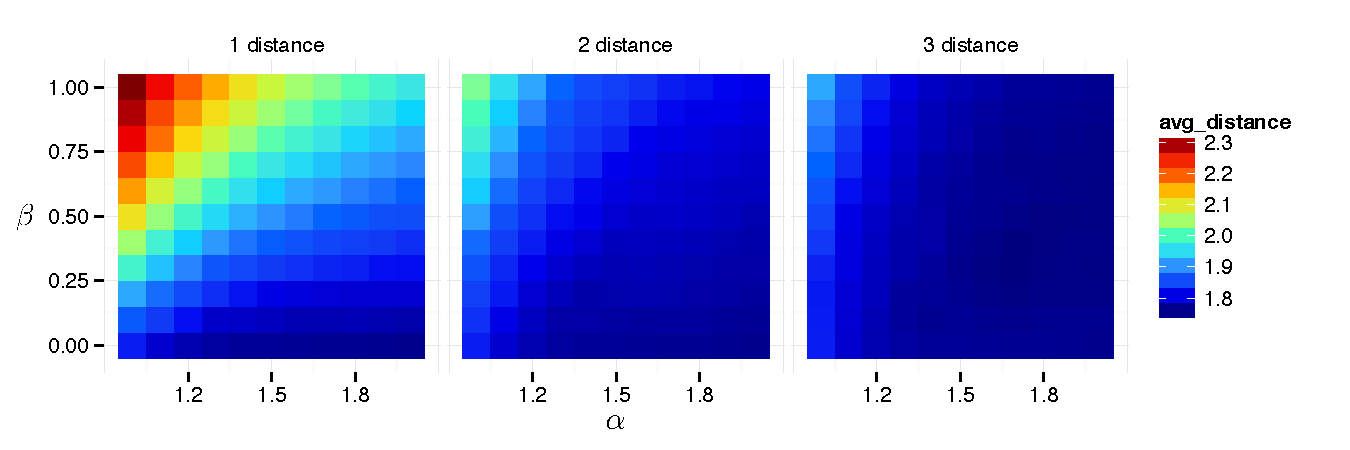
\includegraphics[width=4.0in]{images/alpha_beta_relation_plot}\\
\tiny{Finding best parameters to weigh relevant and non-relevant votes}
\end{figure}

Best combination of parameters for non-relevant posters is $\alpha=1.8$ and $\beta=0$

\end{frame}


\begin{frame}{\textbf{Parameter Optimization: algorithm comparison}}

Select one and more relevant posters from same human curated topic

\begin{figure}
\includegraphics[width=2.5in]{images/performance_vs_votes}\\
\tiny{Comparison of algorithms as they learn more from a simulated user}
\end{figure}

Keywords improve suggestions but Science concierge significantly improves upon that. The more votes, the closer distances to human curated topic.

\end{frame}


\begin{frame}{\textbf{Parameter Optimization: algorithm comparison}}

Select two posters with tree distance in human curated from 0 to 3, find topic distance using keywords and abstracts

\begin{figure}
\includegraphics[width=2.5in]{images/human_vs_topic_distance}\\
\tiny{Relationship between human curated distance and topic distance induced by the keyword and Science Concierge models}
\end{figure}

Spearman rank correlation of the Science Concierge and keywords are $\rho=0.442$, $\rho=0.164$ ($p < 0.001$).

\end{frame}